%% LyX 2.1.1 created this file.  For more info, see http://www.lyx.org/.
%% Do not edit unless you really know what you are doing.
\documentclass[english]{scrartcl}
\usepackage{ae,aecompl}
\usepackage[T1]{fontenc}
\usepackage[latin9]{inputenc}
\usepackage{float}
\usepackage{graphicx}
\usepackage{babel}
\begin{document}

\section{Pattern Component Modeling}

Our final analysis was a implementation of a pattern component modelling
(PCM) approach to factorial multivariate analysis, using the cross-validated
mahalanobis distance \cite{waltherrepresentational}. Briefly, we
tested whether the dissimilarity matrix of observed activity patterns
could be decomposed into a linear combination of contrast matrices
generated from our factorial design. Each hypothesis matrix (contrasts
matrices corresponding to our factors, such as main effects and interaction)
was tested for its ability to explain unique variance in the dissimilarity
matrix (or here, the estimated second-moment matrix) using an ordinary
least squares regression. While we have described how PCM is formally
equivalent to the CVMANOVA approach, it has unique advantages in terms
of the simplicity of its implementation.


\subsection{Representational Similarity Analysis (RSA)}

RSA is an method for quantifying the pairwise similarity of patterns
of voxel activity between experimental conditions \cite{kriegeskorte2008representational}.
Unlike multi-voxel classification \cite{haxby2001distributed}, which
test the performance of machine-learning classifiers categorize conditions
on the basis of multi-voxel activity patterns, contemporary RSA allows
for the ratio-scale measurement of pattern similarity, producing more
reliable estimates of condition-specific patterns of activity \cite{walther2015reliability}.
Here, we implemented the cross-validated squared Mehalanobis distance
(or, Linear Discriminant Contrast; LDC) as our measure of pattern
similarity, as it allows for an unbiased estimate of the true distance
between patterns, i.e., the expected value is zero when the true patterns
are identical \cite{waltherrepresentational}. Previous work has found
this distance measure to be more reliable and noise-tolerant than
other measures of pattern similarity, such as correlation distance
and non-cross-validated squared Mehalanobis distances \cite{walther2015reliability}.
It should be noted that while the analysis we implemented is technically
the cross-validated Euclidean distance, these measures are equivalent
when there is no spatial covariance, as was the case in our simulation.
The LDC between conditions i and j over M runs is defined as,

\begin{center}
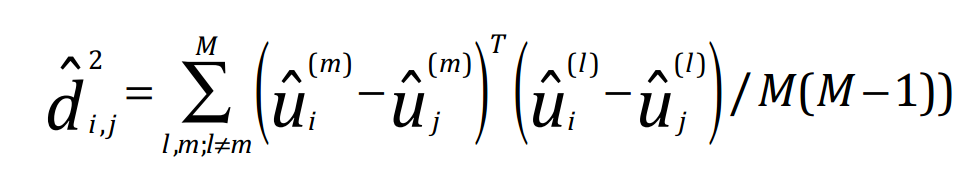
\includegraphics[scale=0.22]{LDC}
\par\end{center}

Where u hat is a vector of voxel activity estimates for each condition
(typically beta weights from a first-level general linear model),
taken from runs m and l. From this matrix of dissimilarity matrix,
we can generate the second-moment matrix (or, G matrix), which includes
an estimate of the variance of each condition\textquoteright s activity
pattern. This is necessary for estimating condition-unique patterns
for the interaction factor. The G matrix can be derived from the LDC
matrix by centring with respect to the mean pattern across conditions.
Using the LDC matrix D, for k conditions,

\begin{center}
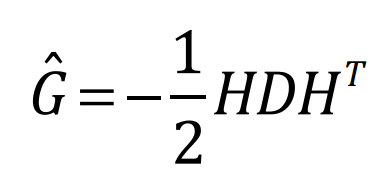
\includegraphics[scale=0.22]{LDCD}
\par\end{center}

where

\begin{center}
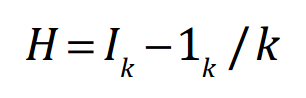
\includegraphics[scale=0.28]{H}
\par\end{center}

The $G$ matrix can also calculated independently from the LDC, as
the variance-covariance matrix of activity patterns over conditions,
a complementary (if not simpler) approach to to the one taken in this
experiment.


\subsection{Pattern Component Modelling (PCM)}

PCM tests whether an observed dissimilarity matrix can be decomposed
into a hypothesized set of independent components. In this case, we
used multiple linear regression to estimate the weight matrix that
that minimized the squared difference between our simulated $G$ matrix
and a set of factorial contrasts. This analysis assumes that our components
are orthogonal, an assumption that is reasonable for random vectors
(i.e., activity patterns) in high-dimensional space. For c contrasts
H1 \dots{} Hc, we estimate the weight matrix $b_{c}$ that minimizes
the difference between our basis matrices $G_{c}$ and our observed
$G$ matrix,

\begin{center}
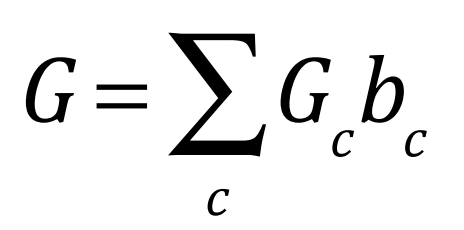
\includegraphics[scale=0.2]{Gmatrix}
\par\end{center}

where 

\begin{center}
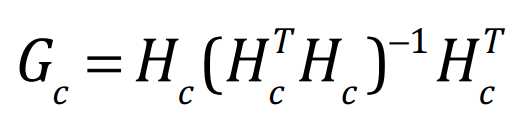
\includegraphics[scale=0.22]{Gc}
\par\end{center}

and 

\begin{center}
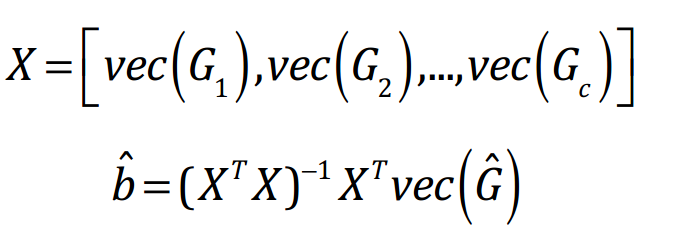
\includegraphics[scale=0.25]{Xb}
\par\end{center}

where the vec operator strings these matrices out into a vector. For
this experiment, our contrasts correspond to the full factorial design:
two main effects and and their interaction (see Figure \ref{fig:Schematic-of-PCM}).
While the interaction contrast is not independent of the main effects
(as addressed in the previous methods), the calculation of these matrices\textquoteright s
pseudoinverse orthogonalized these contrasts in order to estimate
the unique contribution of each contrast for the prediction of the
dissimilarity matrix.

\begin{center}
\begin{figure}[H]
\centering{}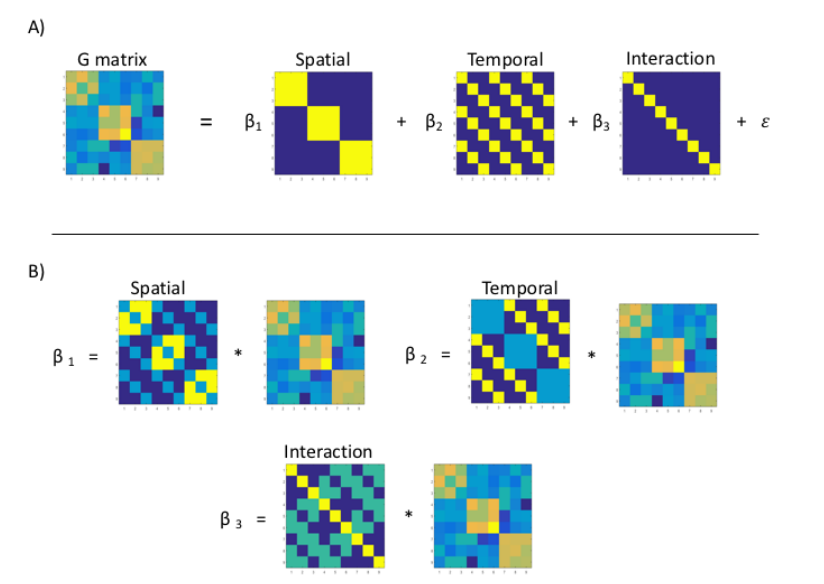
\includegraphics[scale=0.75]{GH}\protect\caption{Schematic of the pattern component model used in this experiment.
A) The cross-validated $G$ matrix is shown comprising of a linear
combination of the basis matrices corresponding to the three contrasts
of our factorial design, plus some error. B) The regression weights
in A are shown to be generated using an OLS estimation: multiplying
the pseudoinverse of the set contrast matrices by our estimated $G$
matrix (here, shown separately). We can see that the peudoinverse
of our basis matrices are orthogonal. The basis matrix of the intercept
is not shown.\label{fig:Schematic-of-PCM}}
\end{figure}

\par\end{center}


\section{Results}

We generated 10 000 simulations of datasets containing combinations
of factors (i.e., main effects or interactions) with signal strengths
of {[}0 .05 .1 .15{]} SNR. For each combination of factors, we generated
a null distribution by permuting the order of the conditions within
each run. This provides a less stringent hypothesis test than a model
with all factors but the factor-of-interest included. However, by
examining the false positive rate for the factor-of-interest in all
of our models where it is not present, we can still estimate the contribution
of other factors on (incorrectly) detecting our factor-ofinteract.
We took the 95th percentile of these permuted distributions as our
critical boundary, calculated the proportion of simulations that had
larger regression weights. While our unbiased measure of pattern similarity
can produce negative weights due to noise, signals will always produce
a positive weight, requiring this one-tailed test of significance.
In Figure \ref{fig:PCM2} we show the rate of H0 rejection for a main
effect (A) and interaction (B) regression weight for combinations
of factors with .15 SNR. We can see that the presence of other factors
does not not alter the H0 rejection rejection rate when the factor
is present or absent, allowing us to confidently use the permuted
null distributions. We can see that there is good sensitivity and
selectivity for main effects and interactions at all combinations
of factor effects. In Figure \ref{fig:PCM2} we can see that as the
SNR increases, there are dramatic increases in the sensitivity of
our test.

\begin{center}
\begin{figure}[H]
\centering{}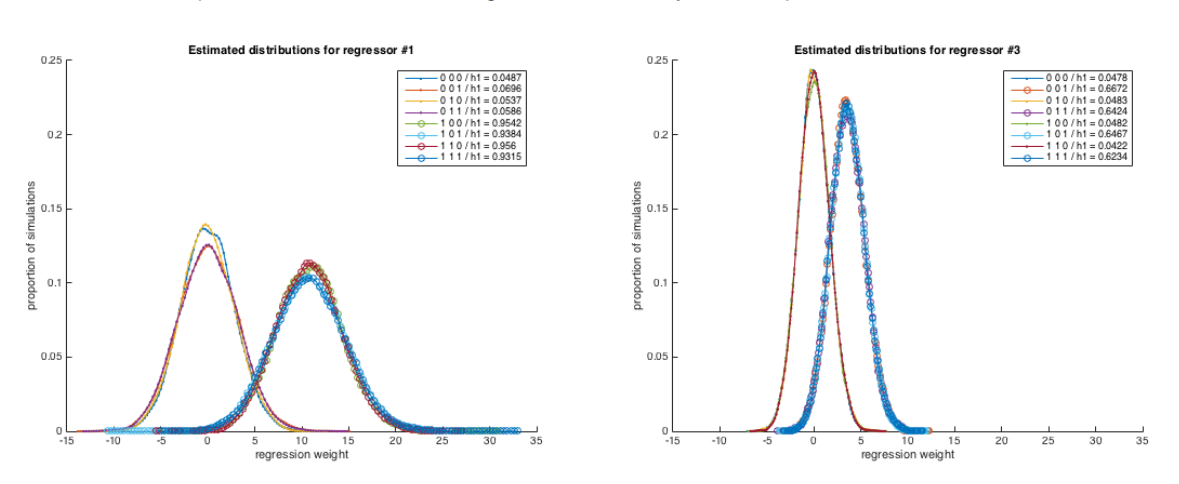
\includegraphics[scale=0.5]{hfig2}\protect\caption{The distributions of regression weights for combinations of factors
at .15 SNR for regressor one (Main Effect) and regressor three (Interaction).
Distributions with unbroken lines are signal-absent trials, and lines
with circles are signal-present trials. There is good sensitivity
and specificity with this approach, regardless of the other factors
present in the simulation, although there is a slight increase in
type 1 error when only interaction effects are present. Legend: (Left)
The combination of 0s and 1s correspond to the absence and presence
of factors, respectively {[}main effect 1, main effect 2, interaction{]}.
(Right) h1 values corresponds to the proportion of simulations with
regression weights greater than the 95th percentile of the permuted
distribution for that combination of conditions.\label{fig:PCM2}}
\end{figure}

\par\end{center}

\begin{center}
\begin{figure}[H]
\centering{}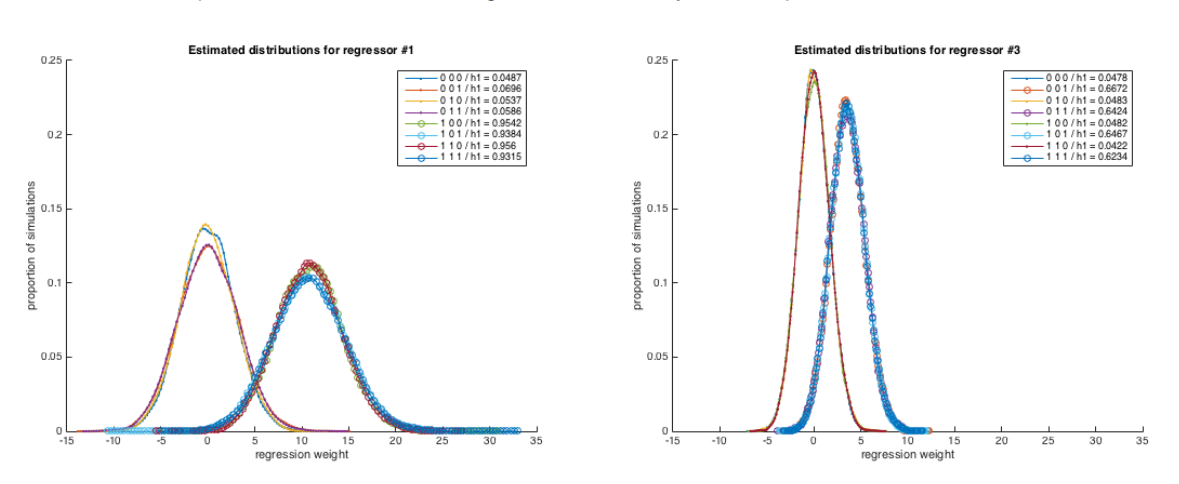
\includegraphics[scale=0.5]{hfig2}\protect\caption{Figure 3. The power of our test at different SNRs for Regressor 1
(main effect) and regressor 3 (interaction). The critical value corresponds
to the 95th percentile of the permuted distribution of the strongest
SNR. As the SNR increases, there is a dramatic increase in power.
Legend: (Left) The SNR of the factor-of-interest. (Right) The power
at that SNR.\label{fig:PCM3}}
\end{figure}

\par\end{center}

\bibliographystyle{unsrt}
\bibliography{ref}

\end{document}
